% This is samplepaper.tex, a sample chapter demonstrating the
% LLNCS macro package for Springer Computer Science proceedings;
% Version 2.20 of 2017/10/04
%
\documentclass[runningheads]{llncs}
%
\usepackage{graphicx}
% Used for displaying a sample figure. If possible, figure files should
% be included in EPS format.
%
% If you use the hyperref package, please uncomment the following line
% to display URLs in blue roman font according to Springer's eBook style:
% \renewcommand\UrlFont{\color{blue}\rmfamily}

\usepackage{amsmath}
\usepackage{amsfonts}
\usepackage{graphicx}
\usepackage{diagbox}
\usepackage{multirow}
\usepackage{booktabs}
\usepackage{float}
\usepackage{url}

\usepackage{color}
\usepackage[all]{xy}
\usepackage{setspace}

\usepackage{geometry}
\geometry{left=2.0cm, right=2.0cm, top=2.5cm, bottom=2.5cm}

\newcommand{\KZ}[1]{\textcolor{blue}{Kenny: #1}}
\newcommand{\tabincell}[2]{\begin{tabular}{@{}#1@{}}#2\end{tabular}}

\begin{document}
	
\renewcommand\arraystretch{1.5}
%
\title{Sentence Alignment of Monolingual Comparable Corpora for Learning Text Rewriting Rules}
%
%\titlerunning{Abbreviated paper title}
% If the paper title is too long for the running head, you can set
% an abbreviated paper title here
%
%\author{Xiwen Chen \and Mengxue Zhang}
%
%\authorrunning{Chen and Zhang}
% First names are abbreviated in the running head.
% If there are more than two authors, 'et al.' is used.
%
%\institute{Advanced Data and Programming Technology Lab \\
%	Computer Science Dept. \\
%	Shanghai Jiao Tong University, 800 Dong Chuan Rd. \\
%	\url{https://adapt.seiee.sjtu.edu.cn/}\\
%	\email{\{victoria-x, lovealice\}@sjtu.edu.cn}}
%
\maketitle              % typeset the header of the contribution
%
\begin{abstract}
Monolingual parallel corpus is crucial for training and evaluating text rewriting models. In order to get rid of inefficient human annotation of monolingual parallel corpus, we explore and devise multiple sentence alignment schemes based on various kinds of unsupervised similarity measures. Based on the paraphrase detection performances of the measurements, we verify that our unsupervised measure is comparable with state-of-art similarity measurements. We use a greedy alignment scheme to ensure quality of aligned pairs, and compare the results with our baselines and a state-of-art alignment model (Bleualign). While our schemes demonstrate comparable alignment efficiency, they are more robust on corpora with special linguistic features. The goal of this work is to construct a monolingual parallel corpus from stylized literatures for learning and evaluating text rewriting rules, especially in style transfer.

\keywords{Monolingual parallel corpora  \and Sentence alignment \and Unsupervised algorithms.}
\end{abstract}
%
%
%
\section{Introduction}
\label{sec:intro}

In natural language processing, there are many supervised learning models that require the existence of parallel corpus for training. However, manual annotation, which is used in constructing many reliable parallel corpora, is inefficient and time-consuming. Multilingual sentence alignment has been extensively studied for machine translation, but the construction of monolingual parallel corpus is also gaining its interest. Monolingual parallel corpora can be used to learn text rewriting rules, which is involved in sentence simplification, natural language style transfer, and document summarization~\cite{hwang2015aligning}. It can also be used to learn the relation of monolingual texts such as semantic relatedness and similarity.

\KZ{Why don't you define the input as two pieces of text, where each text is
a sequence of sentences?}
The monolingual sentence alignment model takes two comparable monolingual 
corpora as an input, and outputs a $x$-to-$y$ alignment of these two corpora, 
where \KZ{the sequential combination of $x$ sentences from the first corpus is 
aligned with $y$ sentences from the second corpus}, 
and both combinations are ``similar'' in content. 
\KZ{The above definition is not clear. You need a figure to illustrate it.}
One implication in this problem statement is that, since the ultimate goal 
is to align two texts to construct parallel corpus, 
only unsupervised methods can be used because we do not have 
pre-aligned examples for training. \KZ{This is not necessarily true. 
Maybe you can say that the motivation to use unsupervised is because there's
insufficient amount of parallel data to train from. But still, you can
annotate yourself.} 

Therefore, the task is divided into two sub-tasks. 
First, we need a measure of similarity for each candidate pair of sentences. 
Second, given two sequences of sentences and a certain similarity measure, 
we need to align the sentences in their original orders according to a 
corresponding global objective.\KZ{The above is not clear..}

The challenge of this task is two-fold. First, similarity measure, which is crucial in alignment decision, is difficult to design for different corpora with different semantic features. \KZ{Second, in each aligned pair, the number of successive sentences in each side is not predetermined but is rather figured out in the sequential alignment process.} Moreover, some similarity measurements that work well for semantic relatedness testing work relatively slow when aligning large corpora. Therefore, the similarity measure for every possible pair and every possible sequential length cannot be viewed as an existing knowledge, leading to some reasonable assumptions of the corpora to ensure efficiency. 

\KZ{Any previous attempts/approaches to solve this problem? What are their
weaknesses?}

The objective of this study is to construct a monolingual comparable corpus with high quality. The corpus can be used in text simplification, style transfer, text summarization, paraphrase detection, and other models that need to learn text rewriting rules. Based on these purposes, the main concern of the model is the quality of the aligned pairs, but not the quantity of them. Namely, an overall optimal solution is not necessarily ensured in the sequential alignment process.

In this paper, we experiment similarity measures based on Word2Vec model~\cite{mikolov2013distributed}, Universal Sentence Encoder~\cite{cer2018universal} and InferSent model~\cite{conneau2017supervised}. Then we evaluate the performance of these measures and compare with baseline models for paraphrase detection. In this comparison, we do not limit ourselves in unsupervised methods. With a greedy algorithm and a filter mechanism for sequence alignment, we next compare the performances of our model with baseline sentence alignment models on literature corpora.

\KZ{Itemize your key technical contributions, usually at least 3.}

\section{Related Work}
\label{sec:related}

With several exceptions, the sentence similarity measure task is fulfilled in two general approaches: (a) sentence embeddings or word embeddings are first obtained and similarity score is calculated based on mathematical measure on vector distance, such as normalized Euclidean distance, cosine distance and earth mover's distance, or (b) similarity score is learned by semantic features or distributional statistics.

Based on word embeddings, Zhu et al. constructed a parallel corpus for text simplification using cosine similarity between TF-IDF vectors of sentences~\cite{zhu2010monolingual}. In the improvements of this work, later studies considered more sentence semantic features including sentence ordering~\cite{coster2011learning} and word-level similarity~\cite{hwang2015aligning}. Then Kajiwara et al. used four word-level alignment methods for similarity measure, and constructed a monolingual parallel corpus for text simplification using similarity matrix and a given threshold~\cite{kajiwara2016building}. Hatzlvassiloglou et al. evaluated the incorporation of multiple linguistic features and the combinations of them in text similarity measure~\cite{hatzlvassiloglou1999detecting}.

In explorations of word-level similarities, word vectors mostly relied on pretrained word vectors such as GloVe~\cite{pennington2014glove} and fasttext~\cite{joulin2017bag} pretrained word vectors. Then word-level similarity and multiple word alignment rules are applied to obtain sentence-level similarities. By directly obtaining sentence vectors, other studies focused more on the forms of distance measure for sentence vectors to better capture the real semantic distance~\cite{kajiwara2016building}.

Apart from unsupervised sentence similarity measure, He et al. used convolutional neural networks with multiple pooling types and window sizes of the $n$-gram model, and considered semantic features in different perspectives, to maximize the utilization of sentence information~\cite{he2015multi}. Ji et al. proposed a distributional sentence similarity with discriminative improvements including TF-IDF and TF-KLD~\cite{ji2013discriminative}. Mueller et al. experimented recurrent neural networks with siamese architecture in sentence similarity measure~\cite{mueller2016siamese}.

In sentence alignment task, Zamani et al. modeled the sequential alignment process using integer programming, arguing that a weak similarity measure is compensated by an optimal sequential alignment algorithm~\cite{zamani2016sentence}. Hwang et al. compared a greedy alignment pattern with an ordered alignment algorithm by dynamic programming, and proved the practical priority of the former~\cite{hwang2015aligning}.

Compared with previous works, the contributions of this work are as follows.
\begin{itemize}
	\item A comparison of two subtasks, similarity measure and sentence alignment, is made based on multiple corpus of various types, including standard corpus for paraphrase detection such as Microsoft Paraphrase Research Corpus~\cite{quirk2004monolingual,dolan2004unsupervised} and SICK~\cite{marelli2014semeval}, and also literature works such as Shakespeare scripts. This comparison reveals the pros and cons of different methods, and can serve as a guidance for semantic similarity studies for more general purposes.
	\item In former studies of monolingual sentence alignment, the main focus is limited to text simplification. This work extends the concept of ``text rewriting rules'' to ``styles'' of a particular text. The sources of the corpus mostly come from literature works of different versions, and thus can be used to learn more general rewriting rules such as style transfer. In this study, multiple measures of similarity combined with a greedy sequential alignment algorithm is compared with two baselines, BleuAlign~\cite{sennrich2010mt,sennrich2011iterative}. The two baselines are originally used to align sentences from bilingual comparable corpora.
	\item A parallel corpus for learning text rewriting rules is constructed using the best-performing combination from the previous analysis. The corpus mainly comes from different versions of translation of classical literature, and thus can be used for style transfer and potentially other text rewriting tasks\footnote{The original sources are mainly obtained from \url{http://gen.lib.rus.ec/}}.
\end{itemize}


\section{Methodology}

An overview of the model architecture is shown in Figure \ref{fig:4}. Under the assumption that the two documents have comparable order in sentences, the model aligns the two texts as follows.
\begin{enumerate}
	\item Given a similarity measure $f_1$, the similarity measurement model computes the scores for all possible one-to-one pairs within a certain distance. This distance is defined as \texttt{MAX\_DISTANCE}, and is the maximum relative distance (given by the index of a sentence in the document) between two single sentences that are considered in this stage.
	\item Pairs whose similarity scores are above a given threshold $t$ is appended in the anchor list. The anchors divide the original document into parts that are relatively shorter for later alignment.
	\item For each part between two pairs of anchors, a local alignment algorithm is performed using a certain similarity measure, where we need to group the sentences and then align the groups. Therefore the alignment is not limited to one-to-one, which is the case in the first stage.
	\item Finally, an optional filtering process is performed. This is due to the observation that, including only one kind of similarity measure might result in unreasonable alignment or too strict alignment rules. To obtain a larger aligned corpus while preserving the quality of aligned sentences, an additional similarity measure can be used to perform a filtering stage for sentences that are not successfully aligned in previous stages. In this stage, we only consider one-to-one alignment.
\end{enumerate}

\begin{figure}[htbp]
	\centering
	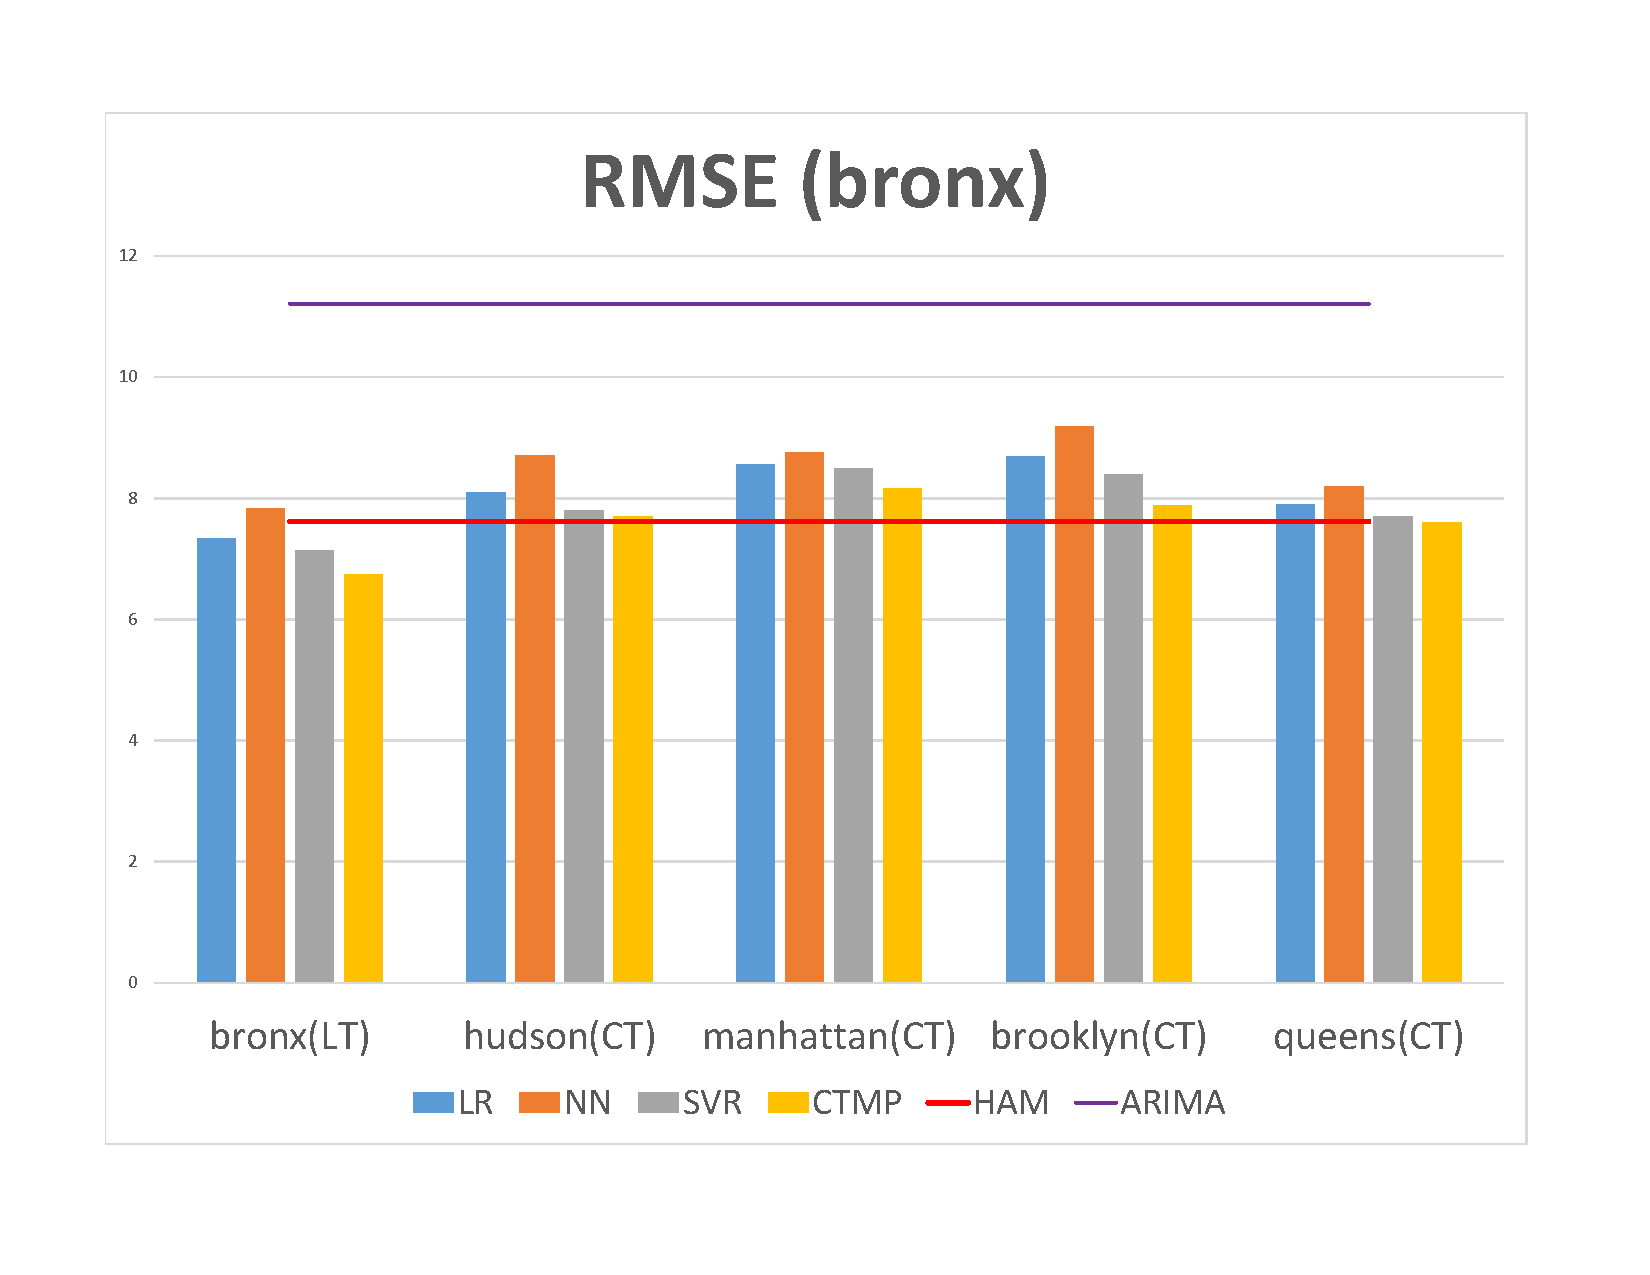
\includegraphics[width=12cm]{./4.png}
	\caption{Model Overview.}\label{fig:4}
\end{figure}

In sum, the model consists of basic similarity measurements and a local sequential alignment in each part separated by successive anchors. The effect of the final filtering stage will also be explored in this work.


\subsection{Similarity Measure}

\KZ{You have to be clear which your method and which are other people's work.
In this section, you should primarily talk about your own methods.}
The first subtask is to give a similarity score for each pair of sentences in order to further align them. In practice, the scoring requires a clustering strategy, since one-to-one sentence mapping is not necessarily required in the sequential alignment task. At this stage, we restrict ourselves to first evaluating the performance of different similarity measures. Namely, given two sentences $(w_1^{(a)}, w_2^{(a)}, \ldots, w_{l_a}^{(a)})$ and $(w_1^{(b)}, w_2^{(b)}, \ldots, w_{l_b}^{(b)})$, where each word in the sequence is a fixed dimensional vector $w_i^{(a)}, w_j^{(b)}\in \mathbb{R}^d$. Then each pair of the sentences $a, b$ gets mapped into a score $r\in [0, 1]$ representing their sentence similarity. The compared models are evaluated based on their accuracies of paraphrase detection task, with corpora including MSRC, SICK, and Shakespeare scripts.

\subsubsection{Supervised Similarity Measure}

Although in our study, supervised similarity measure cannot be deployed, it is still useful to compare the similarity measure we use in the final alignment and the state-of-art sentence supervised methods. The reason is that from practical experiences, the most usual reason for bad performance in alignment is the weakness of similarity measure.

\begin{itemize}
	\item \textbf{Siamese Recurrent Neural Networks (MaLSTM).} This architecture is first proposed by Mueller et al.~\cite{mueller2016siamese}. Utilizing LSTM's priority in learning long range dependencies, they designed a siamese LSTM network (Manhattan LSTM Model) to learn sentence similarity, which is shown in Figure \ref{fig:1}. The sentence is represented as a sequence of fixed-dimensional vectors, which are separately pretrained word vectors from a large corpus. Then the two sentences are fed into two LSTM networks, and the final hidden state is used to calculate the similarity score using a simple distance measure. In their work, the two LSTM networks have the same weights.
	\begin{figure}[htbp]
		\centering
		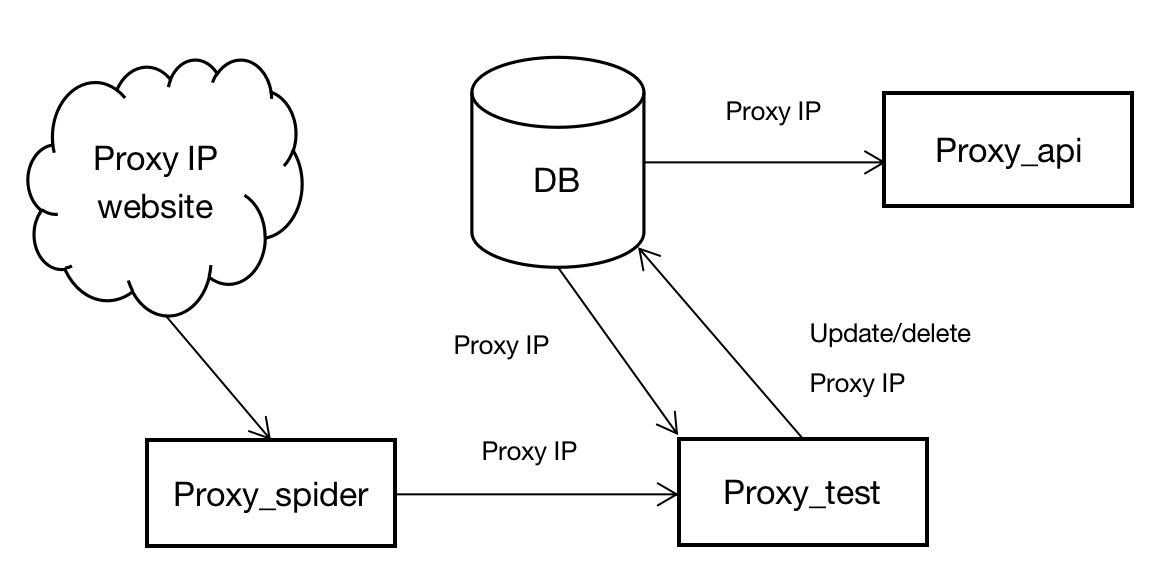
\includegraphics[width=10cm]{./1.png}
		\caption{Manhattan LSTM Model}\label{fig:1}
	\end{figure}
	\item \textbf{TF-KLD.} A discriminative improvement to distributional sentence similarity is proposed by Ji et al.~\cite{ji2013discriminative}. Inspired by the standard TF-IDF (term frequency, inverse document frequency) reweighting approach, which increases the importance of rare words, TF-KLD aims at increasing the weights of discriminative distributional features while decreasing the weights of non-discriminative ones.
	
	Specifically, for each labeled sentence pair, $\langle \vec{w}^{(a)}, \vec{w}^{(b)}, r\rangle$, where $\vec{w}^{(a)}, \vec{w}^{(b)}$ are the distributional features for the two sentences, and $r\in \{0, 1\}$ is the label indicating whether they are paraphrase or not. Then the KL divergence of two Bernoulli distributions,
	\begin{align*}
	p_k & = P[w_{k}^{(a)}|w_{k}^{(b)} = 1, r = 1]\\
	q_k & = P[w_{k}^{(b)}|w_{k}^{(a)} = 1, r = 0],
	\end{align*}
	is given by
	\begin{align*}
	KL(p_k\|q_k) = \displaystyle \sum_xp_k(x)\log \frac{p_k(x)}{q_k(x)},
	\end{align*}
	where $p_k$ represents the probability that the first sentence contains feature $k$, given that $k$ is in the second sentence and the two sentences are paraphrases, and similarly for $q_k$. This KL divergence is then used to reweight the feature vectors for each sentence. Finally, the sample vector $\vec{s}(\vec{v}_1, \vec{v}_2) = (\vec{v}_1 + \vec{v}_2)\oplus |\vec{v}_1 - \vec{v}_2|$, where $+$ and $|\cdot|$ represent element-wise sum and absolute difference, is fed into a Support Vector Machine model to classify as paraphrase and non-paraphrase.
\end{itemize}



\subsubsection{Unsupervised Similarity Measure}

In practice, similarity measures cannot be obtained in a supervised pattern, since we assume there is no labeled one-to-one training corpus for each pair of texts we want to align. Due to this restriction, the general approach for unsupervised similarity measure is composed of a (hopefully strong) sentence representation model and a simple distance measure.
\begin{itemize}
	\item \textbf{Gensim Word2Vec (WDV).} The Gensim implementation of Word2Vec model uses CBOW and Skip-gram models~\cite{mikolov2013distributed}. The two architectures are first proposed by Mikolov et al. While CBOW model predicts the current word based on the context, the Skip-gram model tries to predict the surrounding words given the current word. In our implementation, the word vectors are trained on the two documents to be aligned, rather than using pretrained word vectors given by independent large corpus. This is under the consideration that, since our sentence alignment task is performed on stylized sentences, a corpus-specific Word2Vec model better fits in our scheme. 
	
	After obtaining word embeddings, the sentence embedding is the average of the sum of word vectors in a sentence, or is aligned in a maximizing pattern. To maximize the alignment, each word in sentence 1 is aligned to the most similar word in sentence 2, while each word in sentence 2 is aligned to the most similar word in sentence 1. Then the scores for the alignments in both directions are added and normalized according to sentence length.
	\item \textbf{Universal Sentence Encoder (UNV).} Universal Sentence Encoder proposed by Cer et al.~\cite{cer2018universal} is designed to encode sentences into embedding vectors that specifically target transfer learning. They proposed two models for sentence embedding that are not task specific. The models are obtained from TF Hub.
	\item \textbf{InferSent Model (INF).} InferSent model first proposed as a Facebook research project of learning universal representations of sentences~\cite{conneau2017supervised}. It is based on a bi-directional LSTM with max-pooling (shown in Figure \ref{fig:3}) and trained on the Standford Natural Language Inference dataset~\cite{bowman2015large}, and was proved to be superior to state-of-art models such as SkipThought~\cite{kiros2015skip} and FastSent~\cite{hill2016learning}, as well as other architectures in their study. 
	\begin{figure}[htbp]
		\centering
		
\includegraphics[width=6cm]{./3.png}
		\caption{Bi-LSTM Max-pooling Network.}\label{fig:3}
	\end{figure}
	As is shown in the figure, each hidden state $h_t$ is the concatenation of a forward LSTM and a backward LSTM, and then the hidden states are max-pooled to obtain the final representation. They used GloVe vector as their word embeddings. In our study, we explore both GloVe and FastText pretrained word vectors~\cite{pennington2014glove, joulin2017bag}.
\end{itemize}

Using sentence embeddings, cos and arccos measures are used to calculate the final similarity score, defined as follows.
\begin{align*}
sim_{\cos} & = \cos(v_1, v_2), \\
sim_{\arccos} & = \frac{\arccos(\cos(v_1, v_2))}{\pi}.
\end{align*}


\subsection{Sequential Alignment}

In our scheme of constructing parallel corpus from comparable documents, we need to consider (a) the documents being aligned are potentially large, and (b) there exist sentences that are aligned with two or more sentences from the other document, and also exist sentences that are not aligned at all.

These two possibilities lead to challenges in designing the sequential alignment algorithm, since the grouping of the sentences are not known in advance, the similarity score for each pair of groups is not pre-calculated. Furthermore, exhausting all possible groupings is intractable. Therefore, we make the following assumptions.
\begin{enumerate}
	\item The number of sentences in each group does not exceed a maximum window size \texttt{MAX\_WINDOW\_SIZE} for each part of document. Moreover, to handle the situation of shorter parts, the maximum number of sentences is proportional to a factor, defined as \texttt{SIZE\_PER\_TEN}. The scaled limit 
	$$w_{max} = \texttt{SIZE\_PER\_TEN} \times \texttt{len}(part) / 10$$
	is then compared with \texttt{MAX\_WINDOW\_SIZE}, and the minimum of them is the maximum number of sentences in a group.
	\item Two aligned groups cannot appear farther than a limit \texttt{MAX\_DISTANCE}. The assumption is that the aligned groups in the two documents do not locate far from each other, considering relative distance for the whole document. 
\end{enumerate}

Based on these assumptions, we consider following two approaches.
\begin{itemize}
	\item \textbf{Greedy alignment.} In greedy alignment scheme, between each pair of anchors, the similarity scores for all possible pairs are calculated and sorted in decreasing order. In each selection, the most similar pair is popped from the candidate list, and the remaining groups that include any sentence in the selected pair is deleted from the candidate list. The selection stops until the similarity score for the most similar pair is below a predefined threshold, or there is no pair remaining in the candidate list.
	\item \textbf{Global optimal alignment.} In global alignment scheme, an objective function is defined for each alignment. One choice of such objective function is to require the sum of the similarity scores of all aligned pairs is maximized. Namely,
	\begin{align*}
	a = \arg\max_{a_i} \sum_{p_j} a_i(p_j)s(p_j),
	\end{align*}
	where $a_i(p_j)\in \{0, 1\}$ indicates whether each pair $p_j$ is aligned, and $s(p_j)\in [0, 1]$ is the similarity score for that pair. This subject to an additional restriction that any sentence cannot appear in two aligned groups.
\end{itemize}
We aim at constructing a parallel corpus for text rewriting rules in this study, and thus the main consideration is the quality of aligned groups. Namely, we focus on a local optimization rather than global optimization. Therefore, we proceed with greedy alignment scheme in our work.


\section{Experimental Setup}

\subsection{Similarity Measure}

The similarity measure is evaluated based on a paraphrase detection task performed on Microsoft Research Paraphrase Corpus (MSRC), SICK, and Modern/Original Version of Shakespeare scripts. For supervised similarity measure, experiment is performed directly for each corpus. 

For unsupervised similarity measure, the three sentence embedding schemes with multiple embedding dimensions for word embeddings are combined with the two distance measures, and together with a set of thresholds, are used to label sentences with a similarity score above threshold as paraphrases. We also used BLEU~\cite{papineni2002bleu} and ROUGE~\cite{lin2004rouge}, two popular measures of machine translation quality, as baseline models in this task.

\subsection{Sentence Alignment}

The datasets on sentence alignment are a part of the final documents that are aligned, including \emph{Notre Dame de Paris} and \emph{The Story of Stone}. Related data for each corpus is shown in Table \ref{tb:1}.

\begin{table}[h!]\footnotesize
	\centering
	\small
	\caption{Dataset Lengths.}\label{tb:1}
	\begin{tabular}{|c|c|c|}
		\hline
		Corpus & Translation 1 & Translation 2 \\
		\hline
		Notre Dame de Paris & 10272 & 10179 \\
		The Story of Stone & 46034 & 56256 \\
		\hline
	\end{tabular}
\end{table}

For comparison, a state-of-art alignment method based on machine translation, Bleualign is used to analyze the performances of the interested schemes in this work.

\section{Results}

\subsection{Similarity Measure}

As is mentioned in the previous section, for unsupervised measurements we experiment a set of thresholds and multiple dimensions for word embedding. The result for MSRC with different thresholds is shown in Figure \ref{fig:5}. From the figure we can observe that the highest accuracy is reached by ``WDV + MAX + COS'' at threshold around 0.7, with the second highest accuracy reached by the ``UNV + COS'' combination. 

From the result, it should not be surprising because the paraphrases from MSRC are mostly those with many common words. Then if each word in a sentence is aligned with the most similar word in the other sentence in the pair, it is likely that these two words are the same, i.e., the similarity measures to 1. This gives a high privilege to sentences with many common words, and are labeled as paraphrases, which is the case in MSRC. However, in real alignment situations, it is possible that two sentences do not have many ``common'' words, but rather ``similar'' words, and should be aligned. Therefore, we do not abandon the ``average'' approach in later experiments, since it captures more global information about the words in a sentence.
\begin{figure}[htbp]
	\centering
	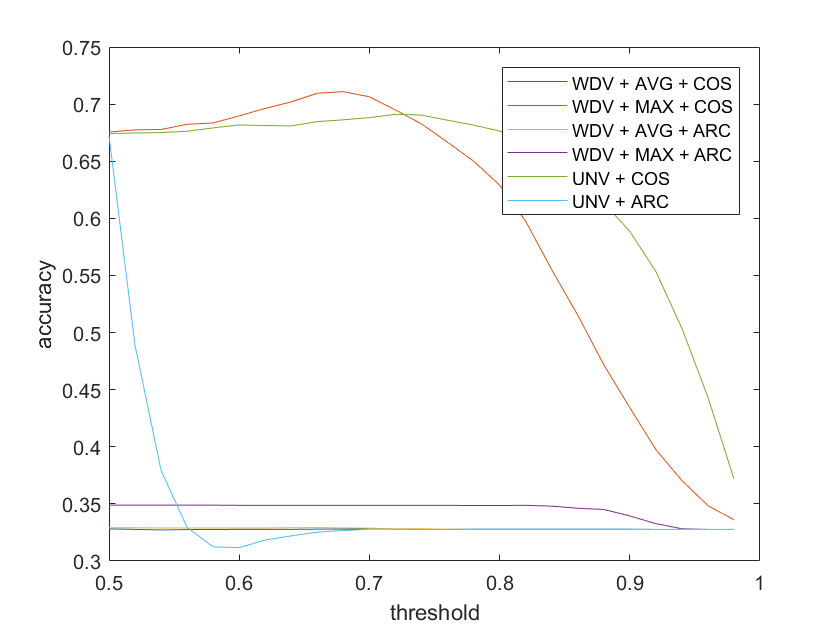
\includegraphics[width=12cm]{./5.png}
	\caption{Accuracies for MSRC with Different Thresholds.}\label{fig:5}
\end{figure}

Another observation is that the cosine measurement is superior to the arccos measurement, which is the case also for SICK and Shakespeare (SHPR). This might be an indication that cosine measure is a more reasonable measure for spatial distance in the vector space of sentence embeddings.

Then for each experimented similarity measurement method, the best dimension for word embedding and the best threshold is used for the final comparison. Since from observations, the accuracies with respect to different dimensions of word embedding do not vary considerably, the dimension is fixed as 100. The results for both supervised and unsupervised methods are shown in Table \ref{tb:2}. (INF-F and INF-G are InferSent models using GloVe and fasttext pretrained word vectors, respectively.)

\begin{table}[h!]\footnotesize
	\centering
	\small
	\caption{Paraphrase Detection Accuracies.}\label{tb:2}
	\begin{tabular}{|c|c|c|c|}
		\hline
		\diagbox{Method}{Accuracy (\%)}{Corpus} & MSRC & SICK & SHPR \\
		\hline
		\hline
		WDV + AVG + COS & 32.8 & 36.6 & 52.5 \\
		WDV + MAX + COS & 71.1 & 68.1 & 72.0 \\
		WDV + AVG + ARC & 32.9 & 36.7 & 53.9 \\
		WDV + MAX + ARC & 34.9 & 39.4 & 54.7 \\
		UNV + COS & 67.9 & \textbf{74.2} & 77.6 \\
		UNV + ARC & 67.2 & 63.5 & 50.0 \\
		INF-F + COS & \textbf{72.2} & 72.5 & \textbf{78.6} \\
		INF-F + ARC & 67.2 & 63.5 & 50.6 \\
		INF-G + COS & 70.4 & 73.0 & 73.9 \\
		INF-G + ARC & 67.2 & 63.4 & 50.8 \\
		\hline
		MaLSTM & 56.9 & 78.3 & 71.6 \\
		TF-KLD & 70.8 & 74.5 & 86.1 \\
		\hline
		BLEU & 69.9 & 65.9 & 71.0 \\
		ROUGE & 71.3 & 67.8 & 71.8 \\
		\hline
	\end{tabular}
\end{table}

From the results, we can conclude that the similarity measurement ability on both standard paraphrase corpus and literature corpus is competent compared with state-of-art similarity models, and especially, supervised models. Among unsupervised similarity measurement, Universal Encoder and InferSent models outperform other methods analyzed. In the sentence alignment task, the ability to measure sentence similarity and the efficiency of this evaluation should both be considered, since the documents to be aligned might be so large that the sentence encoding model costs a lot of computing resources.

\subsection{Sentence Alignment}

The evaluation of sentence alignment is based on the following considerations.
\begin{enumerate}
	\item \emph{Efficiency.} The time a model takes to align sentences should be reasonable with respect to the number of sentences in the raw documents.
	\item \emph{Percentage of aligned sentences.} Although the main focus of this research is to construct a corpus with high quality, the percentage of aligned sentences should also be considered. Namely, we want to asses how many sentences that should be aligned are actually aligned by the model.
	\item \emph{Quality.} Since it is hard to asses whether each sentence is properly aligned or not, we sample a fraction of aligned sentences and decide whether each pair should be aligned manually. The quality of the alignment is evaluated on the percentage of the pairs that are properly aligned with respect to the total aligned pairs. \KZ{You need to rephrase this. Not clear what you
mean. I think we are talking about n-to-n mapping of sentences. So how the 
human judges tell if an alignment is correct is crucial.}
\end{enumerate}

The results for the models performed on the three corpora are shown in Table \ref{tb:3}.

\begin{table*}[th]\footnotesize
	\centering
	\small
	\caption{Quantitative Results ([1] \emph{Notre Dame de Paris}, [2] \emph{The Story of Stone}).}\label{tb:3}
	\begin{tabular}{|c|c|c|c|c|c|c|c|c|c|c||c|}
		\hline
		\textbf{\diagbox{Result}{Model}} & \textbf{BLEU} & \textbf{INF} & \textbf{WDV} & \textbf{UNV} & \textbf{\tabincell{c}{BLEU \\ UNV}} & \textbf{\tabincell{c}{BLEU \\ INF}} & \textbf{\tabincell{c}{WDV \\ UNV }} & \textbf{\tabincell{c}{WDV \\ INF }} & \textbf{\tabincell{c}{INF \\ UNV }} & \textbf{\tabincell{c}{UNV \\ INF }} & \textbf{Bleualign}  \\
		\hline
		\hline
		Time & 1.9m & 8.4m & 4.5m & 1.7h & 1.8h & 9.8m & 19.4m & 8.1m & 24.8m & 3.6h & \textbf{35.6s}  \\
		Percentage [\%] & 73.7 & 70.9 & 73.7 & 42.2 & \textbf{87.1} & 85.0 & 84.6 & 85.2 & 17.7 & 53.6 & 87.0  \\
		Quality [\%] & 100 & 98 & 100 & 91 & \textbf{100} & 100 & 98 & 97 & 100 & 99 & 98   \\
		\hline
		Time & 19.1m & 14.9m & 10.4m & 7.2h & 1.7h & 1.9h & 1.7h & 1.2h & 3.9h & 3.7h & \textbf{4.5m} \\
		Percentage [\%] & 0.35  & \textbf{72.4} & 9.8 & 9.6 & 33.5 & 19.4 & 41.1 & 54.9 & 48.0 & 19.4 & 23.3 \\
		Quality [\%] & \textbf{100} & 45 & \textbf{94} & 57 & 61 & 79 & 59 & 52 & 52 & 39 &  40  \\
		\hline
	\end{tabular}
\end{table*}

Although the baseline model, Bleualign performs the fastest among the compared schemes, it does not guarantee the quality of aligned sentences. Moreover, since it highly relies on one-to-one alignment, it fails in aligning comparable documents that are not so much alike in the first glance, such as \emph{The Story of Stone}. While our models have comparable accuracies and alignment percentage in normal documents, they can be made more robust than Bleualign model in unusual cases by tuning the parameters combining different set of similarity measures.

\section{Constructing a Monolingual Parallel Corpus}

We then proceed to construct a monolingual parallel corpus using the sentence alignment model. The corpus mainly comes from different versions of translation of literature works. A complete list of information about the aligned works is presented in Table \ref{tb:6}.

To evaluate the quality of the alignment, a sample batch of sentences are selected and decided manually on whether the alignment is reasonable. The number of sampled sentences is proportional to the total number of aligned sentences, and the quality of the parallel corpus is represented by the percentage of ``true positive'' with respect to the total number of aligned pairs. In sum, our work achieves reasonable alignment efficiency and generates high quality sentences for text rewriting.

\begin{table*}[h!]\footnotesize
	\centering
	\small
	\caption{Aligned Corpora.}\label{tb:6}
	\begin{tabular}{|c|c|c|c|c|c|}
		\hline
		\textbf{\diagbox{Corpus}{Information}} & \textbf{Author} & \textbf{Translator} & \textbf{Length} & \textbf{Aligned (\%)} & \textbf{Quality (\%)} \\
		\hline
		\hline
		\multirow{2}{*}{Notre Dame de Paris} & \multirow{2}{*}{Victor Hugo} & Alban Krailsheimer & 10272 & 86.3 & \multirow{2}{*}{99.4} \\
		\cline{3-5} 
		& & I. F. Hapgood & 10179 & 87.0 & \\
		\hline
		\multirow{2}{*}{Les Miserables} & \multirow{2}{*}{Victor Hugo} & Julie Rose & 34145 & 76.4 & \multirow{2}{*}{99.0} \\
		\cline{3-5}
		& & I. F. Hapgood & 34328 & 76.0 & \\
		\hline
		\multirow{2}{*}{The Story of Stone} & \multirow{2}{*}{Cao Xueqin} & Yang Xianyi & 46034 & 9.7 & \multirow{2}{*}{94.0} \\
		\cline{3-5}
		& & David Hawkes & 56256 & 8.6 &  \\
		\hline
		\multirow{2}{*}{The Brothers Karamazov} & \multirow{2}{*}{F. Dostoevsky} & A. R. MacAndrew & 24133 & 58.6 & \multirow{2}{*}{95.3} \\
		\cline{3-5}
		& & Richard Pevear & 20288 & 68.1 & \\
		\hline
		\multirow{2}{*}{Crime and Punishment} & \multirow{2}{*}{F. Dostoevsky} & Michael R. Katz & 14503 & 70.6 & \multirow{2}{*}{93.9} \\
		\cline{3-5}
		& & Richard Pevear & 12938 & 76.2 & \\
		\hline
		\multirow{2}{*}{The Magic Mountain} & \multirow{2}{*}{Thomas Mann} & John E. Woods & 14464 & 83.8 & \multirow{2}{*}{97.6} \\
		\cline{3-5}
		& & H. T. Lowe-Porter & 14231 & 83.8 & \\
		\hline
		\multirow{2}{*}{The Illiad} & \multirow{2}{*}{Homer} & Ian C. Johnston & 7744 & 68.1 & \multirow{2}{*}{72.5} \\
		\cline{3-5}
		& & Robert Fagles & 7237 & 58.5 & \\
		\hline
		\multirow{2}{*}{Don Quixote} & \multirow{2}{*}{Cervantes Saavedra} & John Rutherford & 11902 & 48.5 & \multirow{2}{*}{84.4} \\
		\cline{3-5}
		& & John Ormsby & 9056 & 58.3 & \\
		\hline
		\multirow{2}{*}{Anna Karenina} & \multirow{2}{*}{Leo Tolstoy} & Pevear and Volokhonsky & 21398 & 74.6 & \multirow{2}{*}{99.3} \\
		\cline{3-5}
		& & Rosamund Bartlett & 20971 & 74.5 & \\
		\hline
		\multirow{2}{*}{Madame Bovary} & \multirow{2}{*}{Gustave Flaubert} & Eleanor Marx-Aveling & 6670 & 73.9 & \multirow{2}{*}{97.6} \\
		\cline{3-5}
		& & Margaret Mauldon & 6837 & 72.8 & \\
		\hline
	\end{tabular}
\end{table*}

In particular, we highlight the followings.
\begin{enumerate}
	\item In order to guarantee the quality of the corpus, the percentage of aligned sentences with respect to the original length is not necessarily maximized.
	\item Some aligned pairs contain sentences that are exactly identical. We did not discard them, since in order to learn monolingual text rewriting rules, the projection of some expressions to themselves is also included in the style parameter. However, for training or evaluating semantic similarity models, those sentences might be ignored.
\end{enumerate}




\section{Discussion and Conclusion}

\begin{table*}[h!]\footnotesize
	\centering
	\small
	\caption{Aligned Corpora.}\label{tb:4}
	\begin{tabular}{|c|c|}
		\hline
		\textbf{Model} & \textbf{Misaligned Sentence (False Positive [FP] or False Negative [FN])}  \\
		\hline
		\hline
		Bleualign [FP] & \tabincell{c}{\emph{baoyu clapped his hands in approval.} \\ \emph{you're getting quite a temper lately, master bao.}}  \\
		\hline
		BLEU [FN] & \tabincell{c}{\emph{xiang-yan and bao-chai were present that day, it was true; but the absence of...to burst into tears.} \\ \emph{seeing xiangyun and baochai there but not...wanted to take off some clothes.}}  \\
		\hline
		INF [FP] & \tabincell{c}{\emph{the priest whom the girls had noticed...was indeed archdeacon claude frollo.} (31 words) \\ \emph{but she has three things...hands by squeezing her waist.} (79 words)}  \\
		\hline
		WDV [FP] & \tabincell{c}{\emph{what's at stake here are the women.} \\ \emph{are there women or are there not?}} \\
		\hline
		UNV [FP] & \tabincell{c}{\emph{the mob repeated with a frenzied cheer.} \\ \emph{and among the monsters thus...in front of a candle.} (48 words)}  \\
		\hline
	\end{tabular}
\end{table*}

From Table \ref{tb:3} we can conclude that performances of models based on word-level similarity, such as BLEU and Word2Vec model, are in general better than those based on sentence-level similarity, such as InferSent and Universal Sentence Encoder. This is the case when the two comparable documents are already discriminate on word level. In fact, when involving different versions of literature work, it is enough to identify paraphrases based on common or similar words.

In ``special'' documents such as \emph{The Story of Stone}, one-to-one alignment is not necessarily the case, and there are many expressions that might be related to cultural differences. Moreover, some words may represent the same meaning in the specific context, but not in a general sense. Sentence-level semantic similarity might take a more important role in these situations, where methods that are merely based on words might fail to recognize correct alignments.

As a qualitative analysis, we take a few representative sentences from the results that are not properly aligned by different models in the experiment, as is in Table \ref{tb:4}. Although only one pair of sentences is taken for each model, it is selected based on typical misbehaviors of the models. One observation is that word-based alignment schemes, such as BLEU, WDV, and the Bleualign model, is not competent in handling short sentences, while sentence-based alignment schemes fail in cases of longer sentences.

This can serve as an argument for involving similarity measurements from both perspectives. Furthermore, word-level similarity measures can serve as better anchors in the first stage of our model, and sentence-level similarity measures serve well as filters in the second stage. This prevents unreasonable averaging the sentences vectors within a window to ensure efficiency in the first scheme, since sentence level encoders normally takes longer time to embed sentences in every single run.

In sum, we made a comprehensive analysis of similarity measures, and demonstrated the competence of unsupervised methods, which are then used for sentence alignment. We experimented multiple alignment schemes and compared the quality and efficiency with state-of-art alignment model. We then constructed a parallel corpus from different versions of literature works. This corpus can serve as a high-quality learning source or an evaluation set for text rewriting rules, especially for text style transfer.


\bibliographystyle{splncs04}
\bibliography{lncs}



%
% ---- Bibliography ----
%
% BibTeX users should specify bibliography style 'splncs04'.
% References will then be sorted and formatted in the correct style.
%
% 
%

\end{document}
